\documentclass[a4paper]{article}

%% Language and font encodings
\usepackage[english]{babel}
\usepackage[utf8x]{inputenc}
\usepackage[T1]{fontenc}

%% Sets page size and margins
\usepackage[a4paper,top=3cm,bottom=2cm,left=3cm,right=3cm,marginparwidth=1.75cm]{geometry}

%% Useful packages
\usepackage{amsmath}
\usepackage{amsfonts}
\usepackage{graphicx}
\usepackage[colorinlistoftodos]{todonotes}
\usepackage[colorlinks=true, allcolors=blue]{hyperref}
\usepackage{subfig}
\usepackage{xcolor}

\newcommand{\aw}[1]{{\color{blue} [AW: #1]}}
\newcommand{\jm}[1]{{\color{red} [JM: #1]}}
\newcommand{\ap}[1]{{\color{red} [AP: #1]}}

\title{Non-Periodic Edge States}
\author{Jonathan Michala and Alexander Pierson}

\begin{document}
\maketitle

\section{Background}
\section{Loring Index}
Let $\Psi$ be a state in two dimensions with entries $\Psi_{m,n}$, where $m$ describes location with respect to one dimension (whether that be an $x$-coordinate in $\mathbb{R}^2$ or a cell index along an edge) and where $n$ describes location with respect to the other dimension.
Define $X$ and $Y$ to be an operators that act on a state $\Psi$ in the following way:
$$(X \Psi)_{m,n} = m\Psi_{m,n}, \quad (Y \Psi)_{m,n} = n\Psi_{m,n}.$$
Eigenstates of these operators are localized in their corresponding dimensions.
Therefore, when looking for localized eigenstates of a system whose Hamiltonian is $H$, our aim is to find simultaneous eigenstates of all three operators $H$, $X$, and $Y$.\\
This is not always possible, however.
Suppose $A_1,...,A_n$ are Hermitian matrices that all commute with each other.
Then, they can be simultaneously diagonalized, i.e. $U^\star A_i U$ is diagonal for all $i \in \{1,...,n\}$ for some unitary matrix $U$.
So if $H$, $X$, and $Y$ commute, we can find simultaneous eigenstates of them.
Now, suppose $A_1,...,A_n$ do not all commute, but their commutators are bounded:
$$[A_i,A_j] \leq \delta \quad \forall\; i,j \in \{1,...,n\}$$
for some $\delta$.
If $n = 2$, there must exist some $\widetilde{A}_1, \widetilde{A}_2$ such that they commute and satisfy:
$$||\widetilde{A}_1 - A_1||, ||\widetilde{A}_2 - A_2|| \leq \epsilon(\delta)$$
where $\epsilon(\delta) \ll \delta$ \jm{Is this correct?} and where $||M||$ denotes the largest eigenvalue of $M$.\\
But if $n = 3$, there may or may not exist $\widetilde{A}_1, \widetilde{A}_2, \widetilde{A}_3$ such that they all commute with each other and satisfy:
$$||\widetilde{A}_i - A_i|| \leq \epsilon(\delta), \quad \i \in \{1,2,3\}.$$
This existence holds if and only if
$$\frac{1}{2}\; \text{sig} \begin{pmatrix}
A_3 & A_1 + iA_2\\
A_1 - iA_2 & - A_3
\end{pmatrix} = 0$$
where sig$(M)$ is the signature, or number of positive eigenvalues minus negative eigenvalues, of $M$. This is known as the Bott Index of three matrices.
 \aw{this is impossible if they do not commute, also they are only diagonalizable if Hermitian, hence you are looking for vectors which are simultaneous \emph{approximate} eigenvectors of all 3 matrices} of all three of these matrices, i.e. finding $v$ such that $(X - \lambda_1)v = 0$, $(Y - \lambda_2)v = 0$, and $(H-\lambda_3)v = 0$, for real $\lambda_1,\lambda_2,\lambda_3$. This is equivalent(Annals of Physics ref) to finding near-zero eigenvalues of the matrix
$$B(X - \lambda_1, Y - \lambda_2, H - \lambda_3) =
\begin{pmatrix}
H - \lambda_3 & (X - \lambda_1) + i(Y - \lambda_2)\\
(X - \lambda_1) - i(Y - \lambda_2) & - (H - \lambda_3)
\end{pmatrix}.$$
Thus, if this matrix has an eigenvalue less than a specified norm $\epsilon$, we say that it is in the joint pseudo-spectrum of the given lattice. We can also compute the Loring index of $(\lambda_1,\lambda_2,\lambda_3)$ triples which is defined as the signature of $B$. \aw{Hastings-Loring explains the Loring index a little. The point is that } \\\\
To compute the signature of $B$ efficiently, we use the $LDL^T$ decomposition of $B$. $D$ is a block diagonal matrix with blocks of either size $1 \times 1$ or $2 \times 2$. Let $a$ and $b$ be the number of positive and negative $1 \times 1$ blocks in $D$, respectively. By J.R. Bunch, L. Kaufman (Need ref), the signature of $B$ is equivalent to the signature of $D$ which is $a - b$.
\section{Loring Index in Haldane Model}

In the Haldane Model, $m$ and $n$ are the indices of cells on a hexagonal, atomic lattice, where each cell has two sites, labeled $A$ and $B$.
Thus we define our $X$ and $Y$ operators as follows:
$$X_{i,i} = \left\lfloor \frac{i-1}{2} \right\rfloor \;\text{mod}\;m, \quad\quad Y_{i,i} = \left\lfloor \frac{i-1}{2m} \right\rfloor$$
with $X_{i,j} = Y_{i,j} = 0$ for $i \neq j$. 
We compute the pseudo-spectrum and Loring index on the Haldane model lattice with complex hopping and see that in the topological case, the Loring index behave much like the Chern number: on a lattice with edges, the index is $+1$ on the interior and transitions to 0 across the edge; on a periodic lattice, the index is $+1$ everywhere. In the trivial case we see a Loring index of 0 everywhere on edged and periodic lattices, which is analogous to the Chern number. This is shown in Figure \ref{fig:Loring Haldane}.
\begin{figure}
\centering
\subfloat{{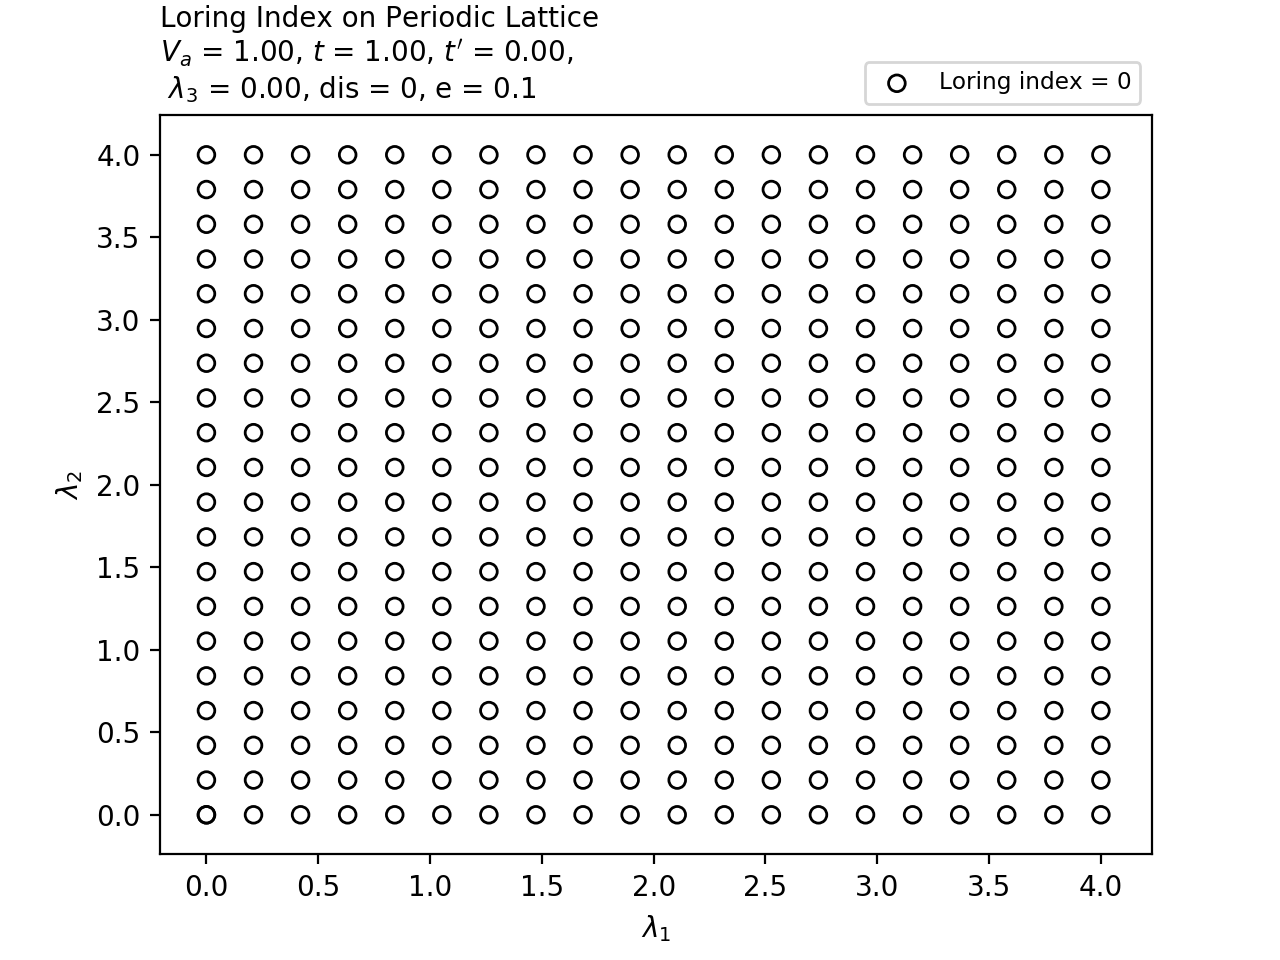
\includegraphics[width=.45\linewidth]{figures/periodic_triv} }}%
\subfloat{{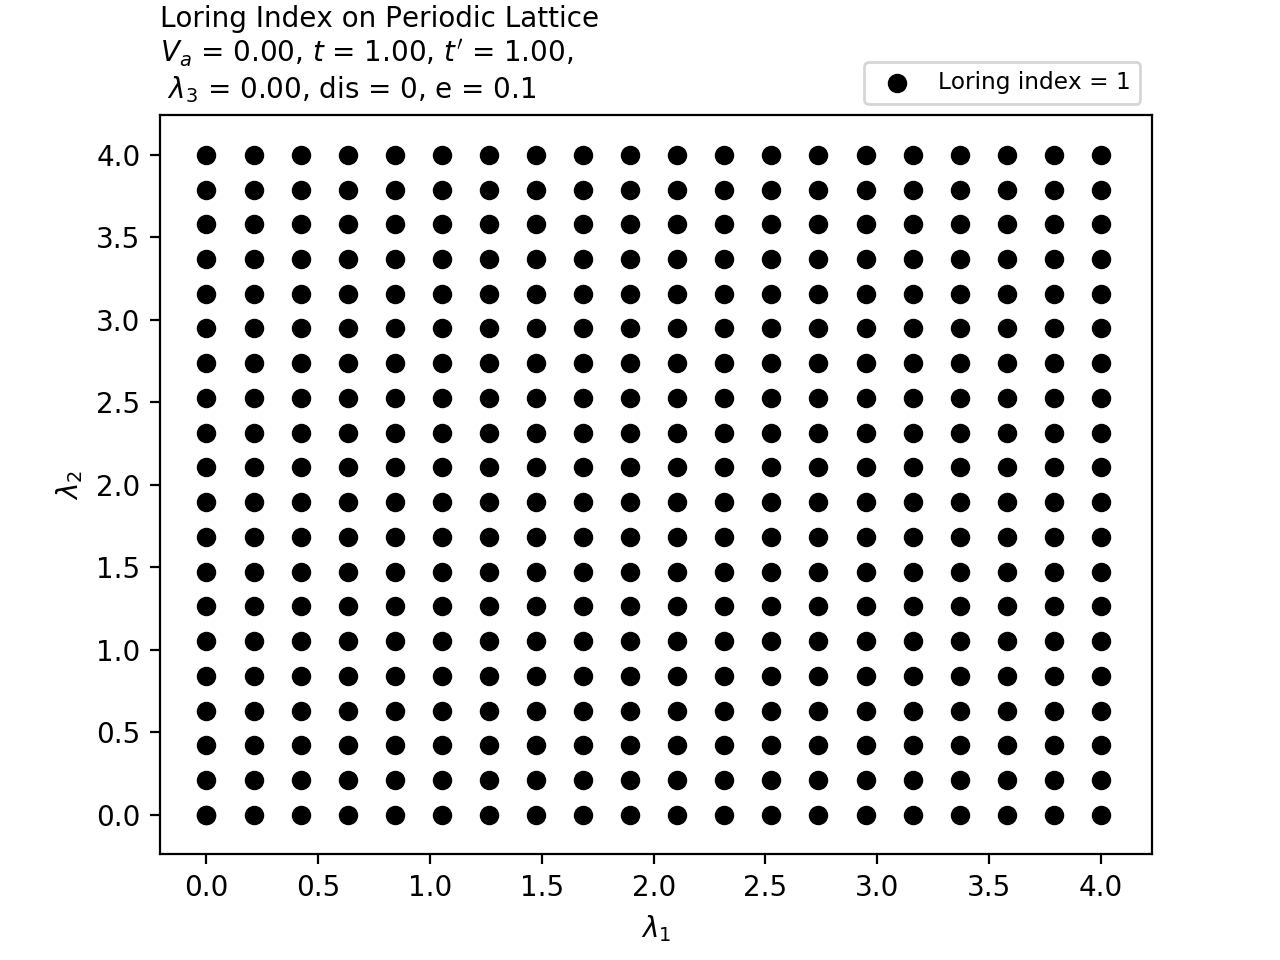
\includegraphics[width=.45\linewidth]{figures/periodic_top} }}%

\subfloat{{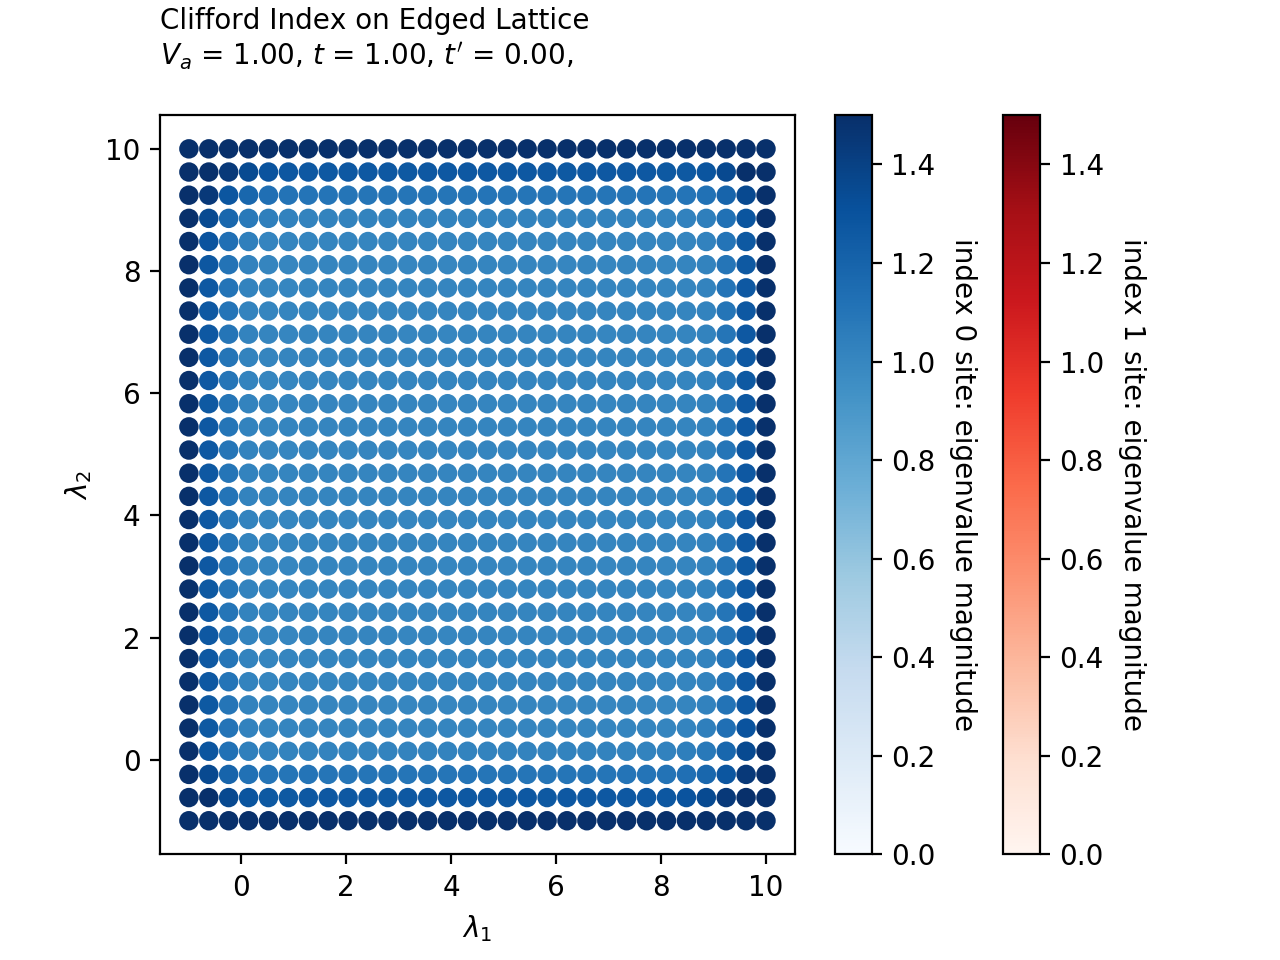
\includegraphics[width =.45\linewidth]{figures/edged_triv} }}%
\subfloat{{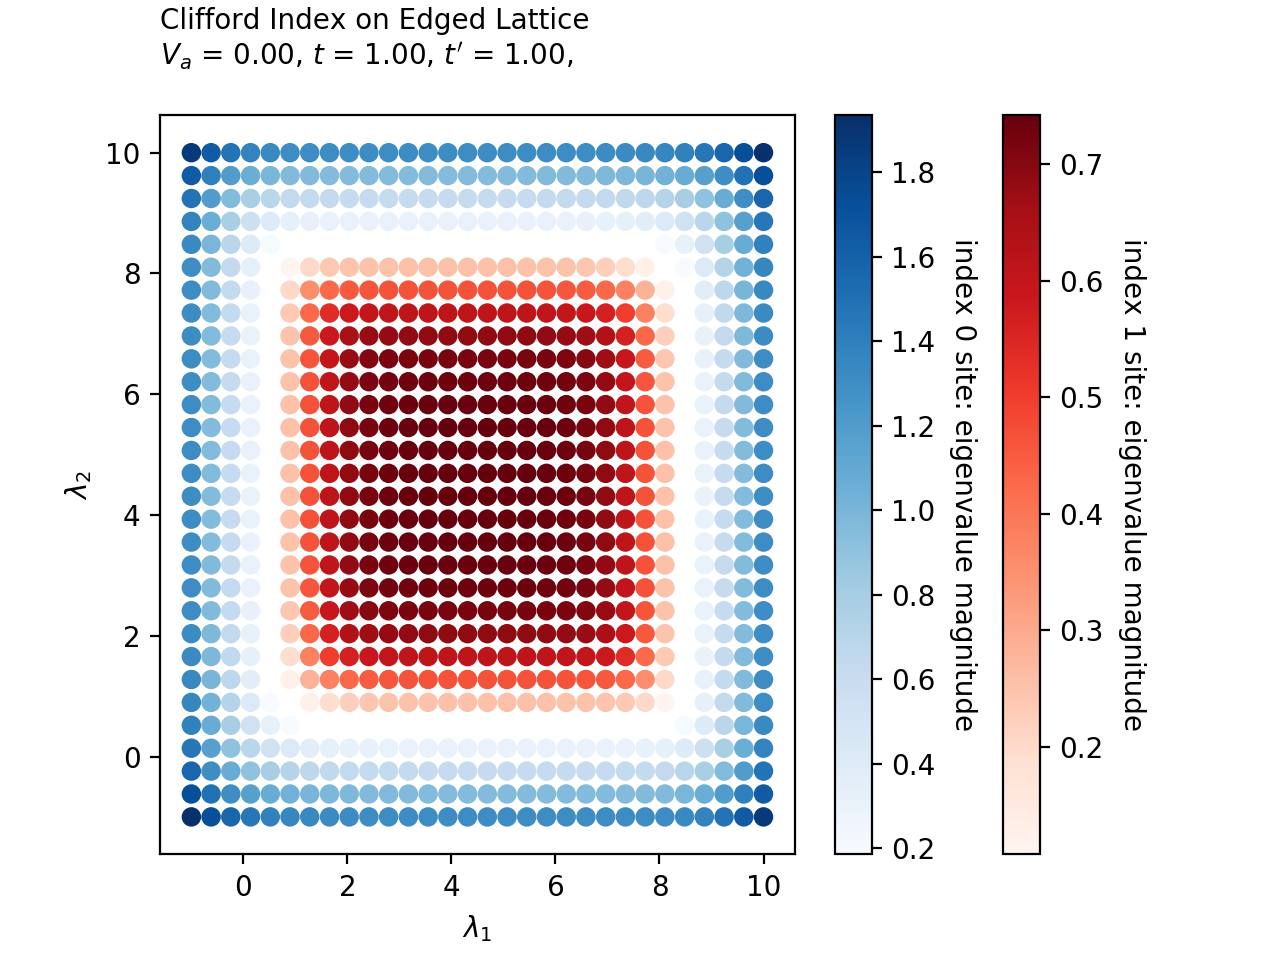
\includegraphics[width =.45\linewidth]{figures/edged_top} }}%
\caption{The top left is a trivial, periodic lattice; the top right is a topological, periodic lattice; the bottom left is a trivial, edged lattice; and the bottom right is a topological, edged lattice. Each site in these figures represents a $(\lambda_1,\lambda_2,\lambda_3)$ triple with $\lambda_3 = 0$. If a site is red, then it is in the pseudo-spectrum, i.e. $B(X - \lambda_1, Y - \lambda_2, H - \lambda_3)$ has a near-zero eigenvalue. If a site is not in the pseudo-spectrum, then it is colored black for Loring index 1 and white for Loring index 0, where the Loring index is defined as the signature of $B$.\\
}%
\label{fig:Loring Haldane}%
\end{figure}
The advantage of the Loring index compared to the Chern number is that the Chern number can only be defined on a periodic structure, whereas the Loring index can be computed on non-periodic media. We will use this advantage to study the robustness of waves on non-periodic media.

\section{Propagation in Haldane Model}
As expected, we find that localized waves propagate along the boundary of the edged, topological lattice since this is a boundary between Loring index 0 and Loring index 1.


\section{\texorpdfstring{$p_x + ip_y$}{px + ipy} Model}
\section{Loring Index in \texorpdfstring{$p_x + ip_y$}{px + ipy} Model}
\section{Propagation in \texorpdfstring{$p_x + ip_y$}{px + ipy} Model}
\end{document}